\section{Lecture 3: Concept and expression of Impostor Terms}

\subsection{Introduction}
Previously, we have talked about ``sampling'' signals, that is, you only ``read'' and ``store'' the value of the signal at certain points. We saw the problems associated with sampling, mainly the fact that given just the sampled signal, it is not possible to reconstruct the original signal, because there are many possible signals which would have given the \emph{same} samples, i.e. they would have taken on the same values as this signal at the points where we are sampling. The natural question to ask, then, is what ``extra information'' do we need in order to reconstruct the original signal from this sample? To do that, we first have to know what these ``other signals'' look like.

\subsection{Non-Uniqueness of Samples}

Previously, we saw graphically that many different sinusoids can have the same samples. We'll now do essentially the same thing, algebraically.

A sinusoid, in general, is of the form $A_0\cos(\Omega_0 t +\phi_0)$, where $\Omega_0 = \frac{2\pi}{T}$, $T$ being the time period, and $\phi_0$ is the initial phase.

Now we saw that the process of sampling was also creating ``ghost frequencies'', frequencies different from that of the original signal, as a side-effect. Of course, these ``impostor terms'', as we can call them, have the same values as the original signal at the point of sampling. We also saw how you can lose a full cycle and arrive at the correct edge, or you only lose half a cycle and arrive at the wrong edge.

Let us represent these ``monster frequencies'' as 
\begin{equation}
\label{eqn:rep}
A_0\cos(\Omega_{kj} t +\phi_{kj})
\end{equation}
Here, $k$ is the number of cycles lost (including the half cycles, if any). $j=1$ signifies that you arrived at the correct edge, and $j=2$ stands for arriving at the wrong edge.

Now suppose we uniformly sample the signal at points $t=nT_s$. We have:
\[x(nT_s)=A_0\cos(\Omega_0 n T_s +\phi_0)\]
Because of the periodicity of the cosine, we can add $\pm 2\pi n k$ to the phase without changing the value of the expression.
\[x(nT_s)=A_0\cos(\Omega_0 n T_s \pm 2\pi nk +\phi_0)
=A_0\cos\left\{2\pi n T_s \left(\frac{1}{T_0} \pm \frac{k}{T_s}\right) +\phi_0\right\}\]
Here, one can think of the term $\frac{1}{T_0}\pm\frac{k}{T_s}$ as the frequency of the impostor in cycles/second, where $k\in \mathbb{Z}^+$.

Now let us assume, for the time being, that we are sampling the sinusoid at least one in each cycle. This is a very reasonable assumption, because if you take less than one sample per cycle, your original sinusoid is itself completing a whole cycle before the next sample is taken. Thus, we assume that $T_0 > T_s$.This would imply that $\frac{1}{T_0}-\frac{k}{T_s}<0$, which says that the frequency is negative, which is something we don't like! But that's not too bad! We know that $\cos$ is symmetric about the $y$-axis. Hence, instead of only one expression with the $\pm$, we write two separate expressions:

\[A_0\cos\left\{2\pi n T_s \left(\frac{1}{T_0} + \frac{k}{T_s}\right) +\phi_0\right\}\]

\centerline{and}

\[A_0\cos\left\{-\left\{2\pi n T_s \left(\frac{1}{T_0} - \frac{k}{T_s}\right) +\phi_0\right\}\right\}=
A_0\cos\left\{2\pi n T_s \left(\frac{k}{T_s}-\frac{1}{T_0}\right) - \phi_0\right\}
\]

Here, the first expression represents that we arrived on the correct edge after skipping $k$ cycles completely, and the second one means that we arrived at the incorrect edge after ``almost'' skipping $k$ cycles. Hence, with respect to the expression (\ref{eqn:rep}) which we wrote earlier, we can say that
\begin{align}
\Omega_{k1}&=2\pi\left(\frac{k}{T_s} + \frac{1}{T_0}\right)  &\phi_{k1}=\phi_0\\
\Omega_{k2}&=2\pi\left(\frac{k}{T_s} - \frac{1}{T_0}\right) &\phi_{k2}=-\phi_0
\end{align}
It is worthwhile to note that the signs of $\frac{1}{T_0}$ and $\phi_0$ match in both expressions.

\begin{figure}[ht]
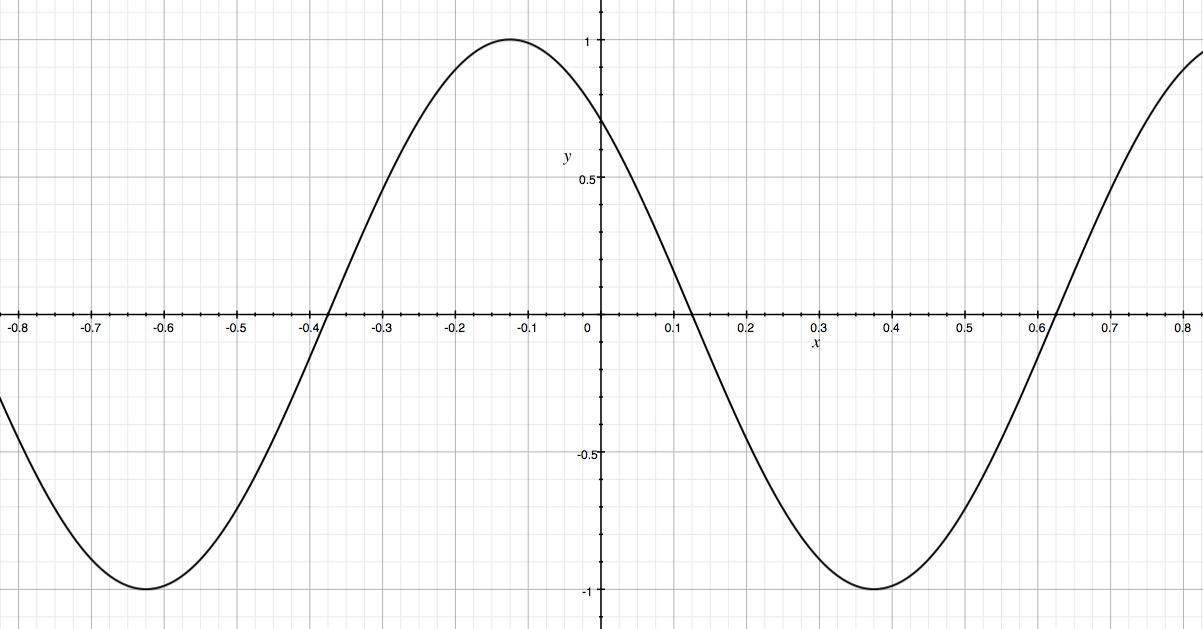
\includegraphics[width=\textwidth]{1-Original}
\caption{\label{fig:originalSignal}The original signal, $y=\sin\left(\frac{2\pi t}{T_0}+\frac{\pi}{4}\right)$}
\end{figure}

\begin{figure}[ht]
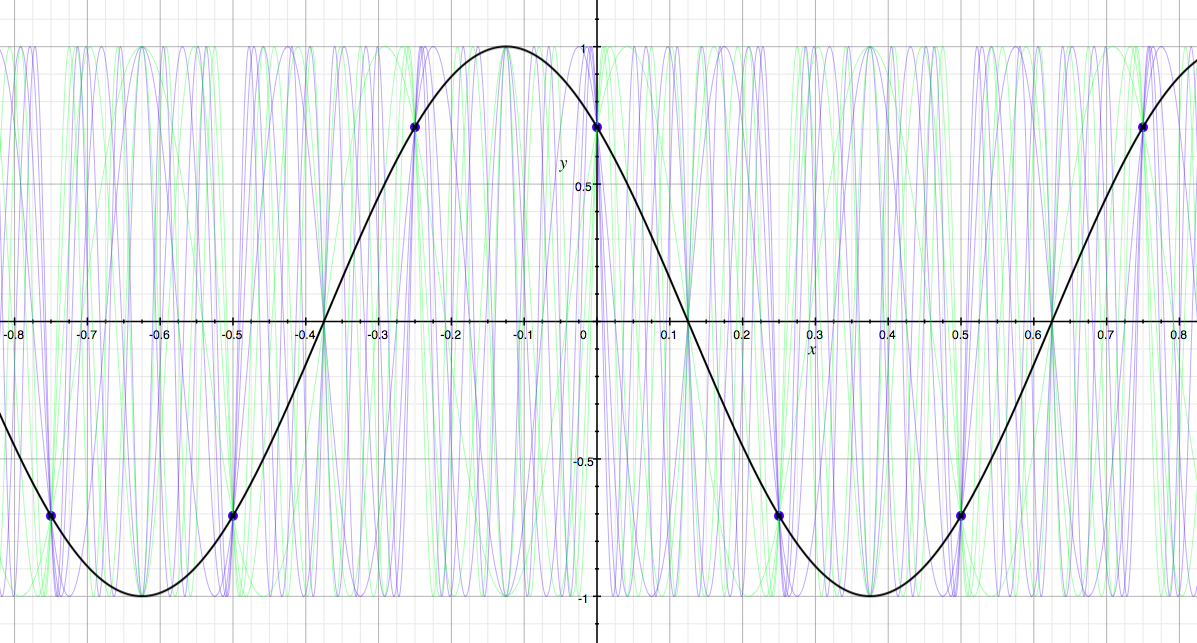
\includegraphics[width=\textwidth]{2-Sampled}
\caption{\label{fig:sampled}The original signal, from Figure~\ref{fig:originalSignal}, sampled at points $t=nT_s , \forall n\in\mathbb{Z}$}
\end{figure}

\begin{figure}[ht]
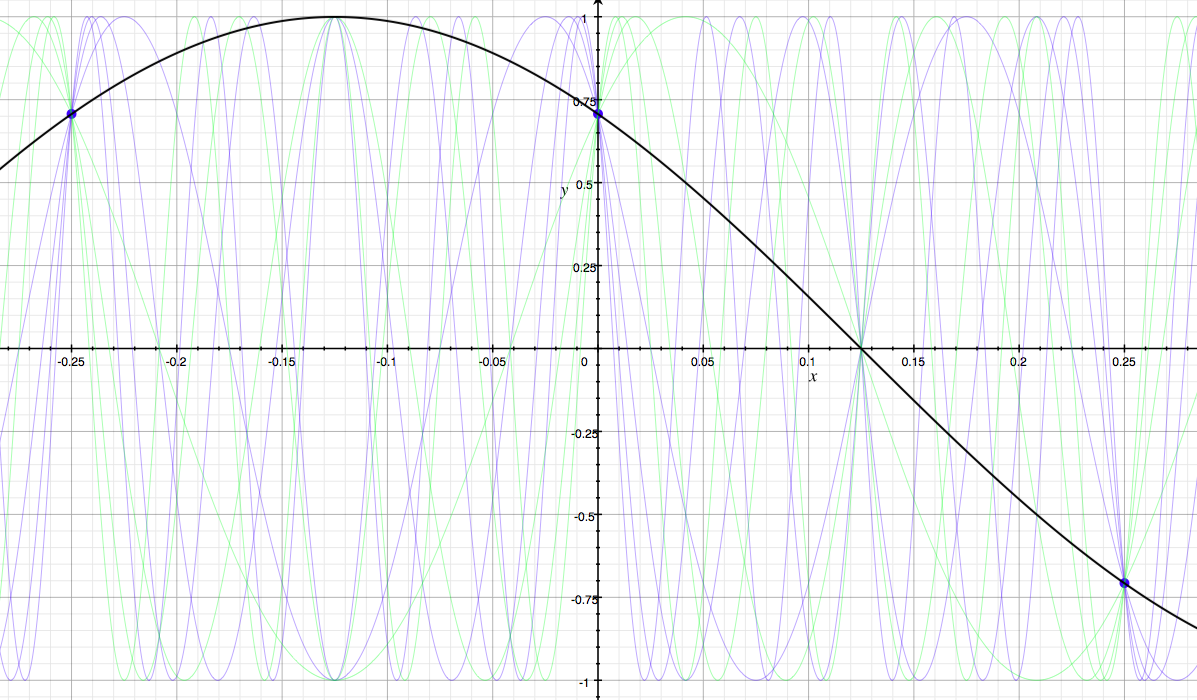
\includegraphics[width=\textwidth]{3-Zoomed_In}
\caption{\label{fig:zoom}Zoomed in view of the same signal}
\end{figure}

\begin{figure}[ht]
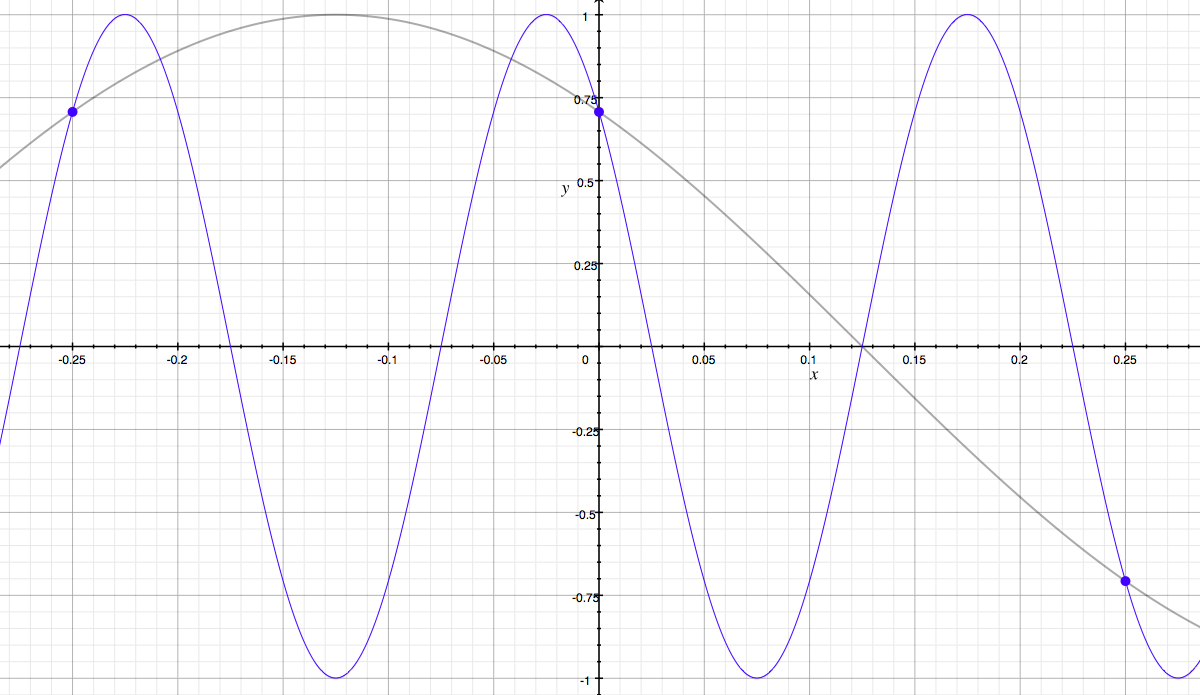
\includegraphics[width=\textwidth]{4-1CE}
\caption{\label{fig:1CE}Missing 1 cycle and arriving at the correct edge}
\end{figure}

\begin{figure}[ht]
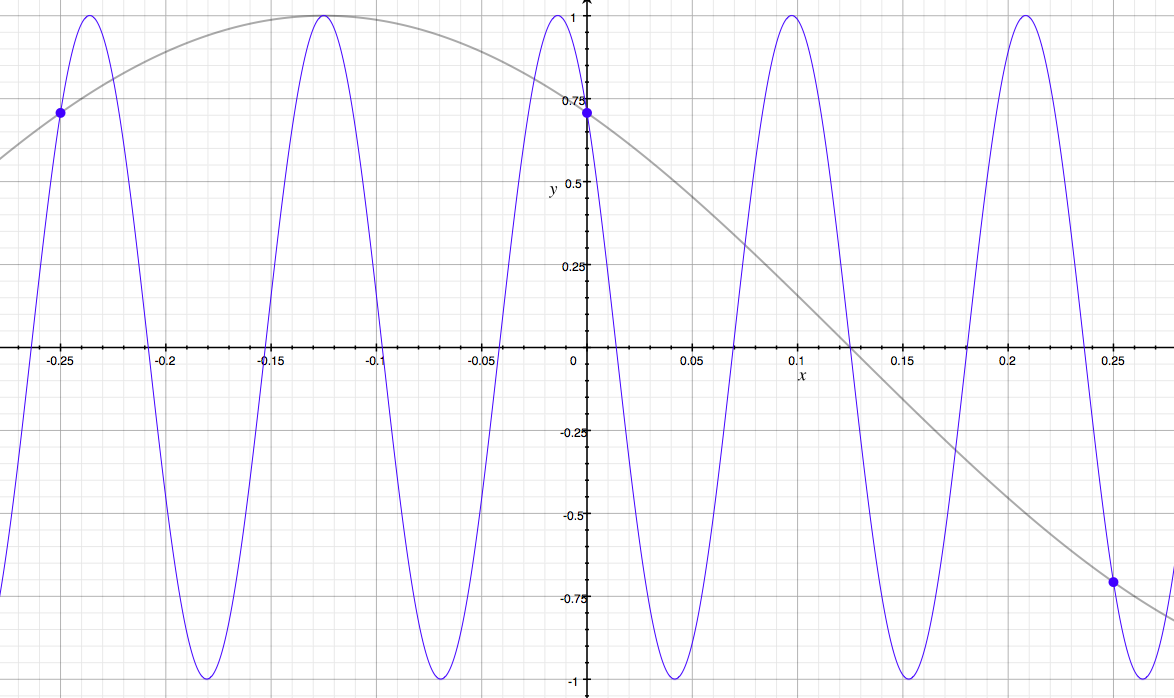
\includegraphics[width=\textwidth]{5-2CE}
\caption{\label{fig:2CE}Missing 2 cycles and arriving at the correct edge}
\end{figure}

\begin{figure}[ht]
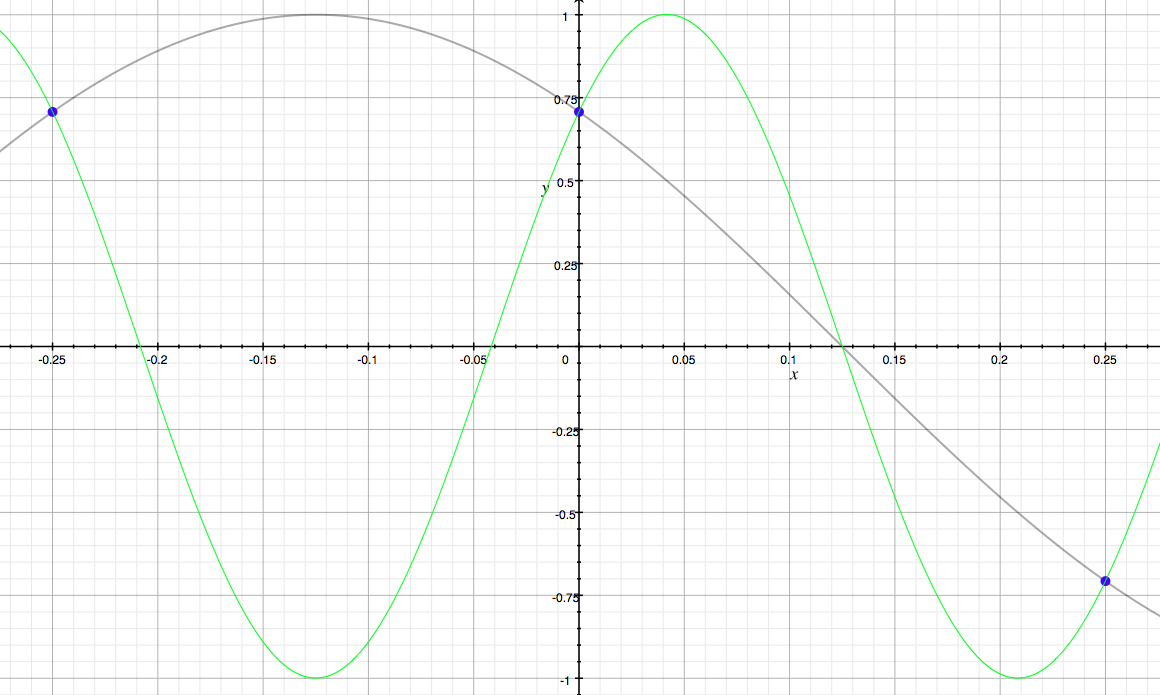
\includegraphics[width=\textwidth]{6-1IE}
\caption{\label{fig:1IE}Missing 1 cycle and arriving at the incorrect edge}
\end{figure}

\begin{figure}[ht]
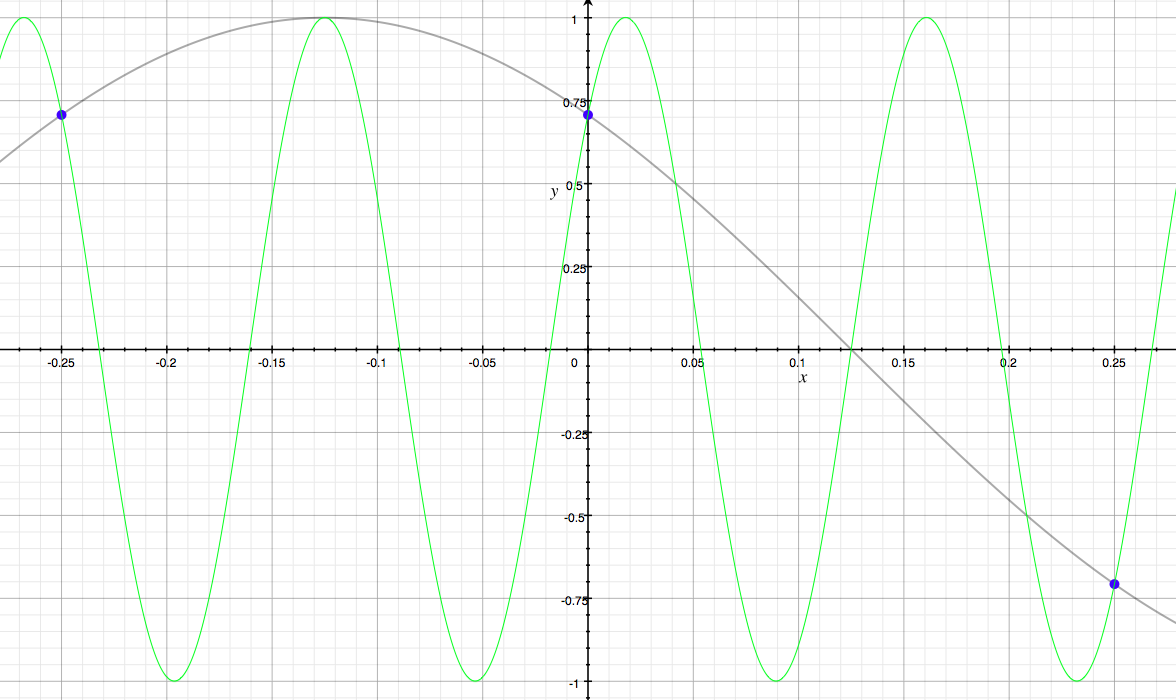
\includegraphics[width=\textwidth]{7-2IE}
\caption{\label{fig:2IE}Missing 2 cycles and arriving at the incorrect edge}
\end{figure}

